%=========================================================
\chapter{Diseño Arquitectónico}
\label{cap:reqUsr}

	Es una etapa clave en el desarrollo del sistema, donde se establecen las bases para su construcción y funcionamiento. En esta sección, se abordarán diversos aspectos relacionados con la arquitectura del sistema, como las propiedades del software, la plataforma utilizada, el costo y la arquitectura misma.

En cuanto a las propiedades del software, se considerarán aspectos como la modularidad, la escalabilidad, la flexibilidad y la fiabilidad. Estas propiedades son fundamentales para garantizar que el sistema pueda adaptarse a cambios futuros, crecer en función de las necesidades del usuario y mantener un rendimiento óptimo en diferentes situaciones.\\

La elección de la plataforma del sistema es otro aspecto importante a considerar. Esto incluye seleccionar el entorno de desarrollo, el lenguaje de programación, las herramientas y los frameworks que serán utilizados para implementar el sistema. La elección adecuada de la plataforma puede tener un impacto significativo en la eficiencia del desarrollo y en el rendimiento del sistema final.

El costo es otro factor crítico a tener en cuenta durante el diseño arquitectónico. Se deben considerar los recursos financieros disponibles, así como los costos asociados con la adquisición de hardware, licencias de software, mantenimiento y capacitación. El diseño arquitectónico debe buscar un equilibrio entre las funcionalidades y características deseadas y los recursos disponibles.\\

En cuanto a la arquitectura del sistema, se definirán los componentes principales, sus interacciones y la estructura global del sistema. Esto implica decidir si se utilizará una arquitectura monolítica, cliente-servidor, basada en microservicios u otra opción. La elección de la arquitectura adecuada dependerá de factores como los requisitos funcionales y no funcionales del sistema, la escalabilidad y el rendimiento esperado.

En resumen, el capítulo de "Diseño Arquitectónico" abarca diversos aspectos fundamentales para el desarrollo del sistema. Se consideran las propiedades del software, la elección de la plataforma, el costo y la definición de la arquitectura. Estos elementos sientan las bases para la construcción de un sistema robusto, eficiente y que cumpla con los requisitos establecidos.


%---------------------------------------------------------
\section{Propiedades del Software.}
En el diseño arquitectónico de un sistema, es importante tener en cuenta diversas propiedades del software que pueden influir en su calidad, rendimiento y mantenibilidad. Estas propiedades abarcan diferentes aspectos del sistema y su comportamiento, y se consideran como criterios clave para evaluar su eficacia y adecuación a los requisitos establecidos.

Algunas propiedades del software relevantes para el diseño arquitectónico del sistema son:

\begin{itemize}
\item \textbf{Escalabilidad de datos}: La escalabilidad de datos se refiere a la capacidad de un sistema para manejar y gestionar grandes volúmenes de datos a medida que crece. Implica diseñar y construir una infraestructura de datos que pueda adaptarse y mantener un rendimiento óptimo a medida que la cantidad de datos aumenta, debido al fácil aumento de reportes por día para cada infante.\
Dentro del sistema se buscó hacer escalable gracias a la base de datos \textbf{Cosmos DB}, que ofrece características y funcionalidades que permiten escalar datos de manera efectiva, ya sea a través de la escalabilidad horizontal, la replicación global, los índices eficientes y la integración con servicios en la nube.

Cosmos DB es una base de datos multimodelo y globalmente distribuida ofrecida por Azure. Permite almacenar y consultar datos de manera escalable y de alto rendimiento, con soporte para múltiples modelos de datos, como documentos, grafos, clave-valor y columnas. Al aprovechar la escalabilidad horizontal, Cosmos DB puede manejar grandes volúmenes de datos y crecer a medida que aumenta la carga de trabajo.

Además, Cosmos DB ofrece replicación global, lo que garantiza que los datos estén disponibles en múltiples regiones geográficas, mejorando la disponibilidad y la latencia de acceso a los datos en todo el mundo. Los índices eficientes permiten acelerar las consultas y mejorar el rendimiento de las operaciones, lo que es crucial para gestionar grandes volúmenes de datos en un tiempo razonable.


\item \textbf{Flexibilidad}: Capacidad del sistema para adaptarse a cambios y requerimientos futuros sin necesidad de realizar modificaciones mayores en la arquitectura. Un diseño arquitectónico flexible permite incorporar nuevas funcionalidades, integrar tecnologías emergentes o adaptarse a diferentes entornos sin comprometer la estabilidad del sistema.

\item \textbf{Seguridad}: La seguridad del software es esencial para proteger los datos, las funcionalidades y los usuarios del sistema. Un diseño arquitectónico seguro debe incluir mecanismos y controles adecuados para prevenir ataques, garantizar la confidencialidad, la integridad y la disponibilidad de la información, y mitigar posibles vulnerabilidades. Para ello es que se han agregado medidas de autenticacion A través del uso de middlewares en Express.js, se pueden implementar mecanismos de autenticación, como \texttt{JSON Web Tokens (JWT)}, para verificar la identidad de los usuarios y controlar el acceso a las funcionalidades del sistema.
Ademas de la gestión de permisos y roles dentro del sistema.

\item \textbf{Rendimiento}: El rendimiento se refiere a la capacidad del sistema para responder de manera eficiente a las solicitudes de los usuarios y procesar grandes volúmenes de datos en un tiempo razonable. Un diseño arquitectónico que optimice el rendimiento debe considerar aspectos como la optimización de algoritmos, el uso eficiente de recursos y la minimización de cuellos de botella.

Para lograr un alto rendimiento en el sistema, se busca implementar una infraestructura en la nube utilizando Azure. Azure es una plataforma de servicios en la nube que ofrece diversas ventajas en términos de rendimiento, escalabilidad y disponibilidad. Algunas de las razones por las cuales se elige Azure son:

\item \textbf{Mantenibilidad}: La mantenibilidad se refiere a la facilidad con la que se puede realizar el mantenimiento y la evolución del sistema a lo largo del tiempo. Un diseño arquitectónico mantenible facilita la identificación y corrección de errores, la incorporación de mejoras y la adaptación a cambios en los requisitos o tecnologías subyacentes. Esto se logró dividiendo cada subsistema en una careta distinta en la REST API, la carpeta \texttt{controladores}, contiene todos los controlladores de cada entidad, y llevan toda las acciones y logica de los usuarios, la carpeta \texttt{modelos} contiene a los objetos creados dentro de la base de datos, la carpeta \texttt{rutas} definen las rutas y la gestión de las solicitudes HTTP de cada entidad.
\end{itemize}

Estas propiedades del software son solo algunas de las muchas consideraciones que deben tenerse en cuenta durante el diseño arquitectónico. La elección adecuada de estas propiedades dependerá de los requisitos y objetivos específicos del sistema, así como de las restricciones y contextos en los que se desarrolla. Al optimizar y equilibrar estas propiedades, se puede lograr un diseño arquitectónico sólido y efectivo que cumpla con las necesidades de la guarderia.


%---------------------------------------------------------
\section{Plataforma}

La plataforma se refiere al entorno o conjunto de recursos tecnológicos utilizados para alojar y ejecutar la aplicación o sistema. En otras palabras, es la infraestructura sobre la cual se implementa y se ejecuta el sistema.

\begin{itemize}
\item \textbf{Cosmos DB}: Es una base de datos multimodelo y globalmente distribuida ofrecida por Azure como un servicio de base de datos como servicio (DBaaS). Cosmos DB permite almacenar y consultar datos de manera escalable y de alto rendimiento. Ofrece soporte para múltiples modelos de datos, como documentos, grafos, clave-valor y columnas, lo que brinda flexibilidad en el diseño de la base de datos según las necesidades del sistema. Además, Cosmos DB proporciona características como la replicación global, la latencia baja y la alta disponibilidad, lo que garantiza un acceso rápido y confiable a los datos en todo el mundo.

\item \textbf{Express.js}: Es un framework de desarrollo web para Node.js. Express.js se encarga de construir la parte del servidor de la aplicación web, permitiendo definir rutas, manejar peticiones HTTP y establecer la lógica de negocio del sistema.

\item \textbf{Vue.js}: Es un framework de JavaScript utilizado para construir la interfaz de usuario y la parte del cliente de la aplicación web. Vue.js facilita la creación de componentes reutilizables y la gestión del estado de la aplicación, lo que mejora la experiencia del usuario y la interactividad del sistema.

\item \textbf{Node.js}: Es un entorno de ejecución de JavaScript basado en el motor V8 de Google Chrome. Node.js permite ejecutar código JavaScript en el lado del servidor, lo que proporciona un entorno coherente tanto en el cliente como en el servidor. Node.js ofrece una amplia gama de bibliotecas y módulos que facilitan el desarrollo de aplicaciones web robustas y escalables.

\item \textbf{Azure PaaS}: Azure Platform as a Service (PaaS) es un conjunto de servicios en la nube ofrecidos por Azure que permite a los desarrolladores construir, desplegar y administrar aplicaciones sin tener que preocuparse por la infraestructura subyacente. Azure PaaS ofrece servicios específicos para el desarrollo y despliegue de aplicaciones web, como Azure App Service, que permite desplegar aplicaciones web basadas en Node.js, Express.js y Vue.js de manera rápida y sencilla.

\item \textbf{Azure DBaaS}: Azure Database as a Service (DBaaS) es un servicio ofrecido por Azure que permite a los desarrolladores utilizar bases de datos en la nube sin tener que administrar la infraestructura subyacente. Azure DBaaS incluye servicios como Cosmos DB, que es una base de datos multimodelo globalmente distribuida. Estos servicios ofrecen escalabilidad, disponibilidad y rendimiento optimizados, lo que facilita el almacenamiento y acceso a datos de manera eficiente en el sistema.

\item \textbf{Azure}: Se utiliza la plataforma en la nube Azure para alojar y desplegar el sistema. Azure proporciona una infraestructura escalable y altamente disponible, lo que garantiza un rendimiento óptimo y una disponibilidad continua del sistema. Además, Azure ofrece una amplia gama de servicios y herramientas que pueden utilizarse para optimizar y mejorar el rendimiento del sistema, como la escalabilidad automática, el equilibrio de carga y la gestión de recursos.
\end{itemize}

La elección de la MEVN stack como arquitectura del sistema, junto con el uso de servicios como Cosmos DB y Azure PaaS, ofrece numerosos beneficios, como la flexibilidad en el manejo de datos, la eficiencia en el manejo de peticiones, la capacidad de crear interfaces de usuario interactivas y una infraestructura escalable y confiable. Esto permite construir un sistema web moderno, escalable y de alto rendimiento.

En la Figura \ref{fig:plataforma} se muestra una representación visual de la plataforma mencionada en operación.

\begin{figure}[htbp]
\centering
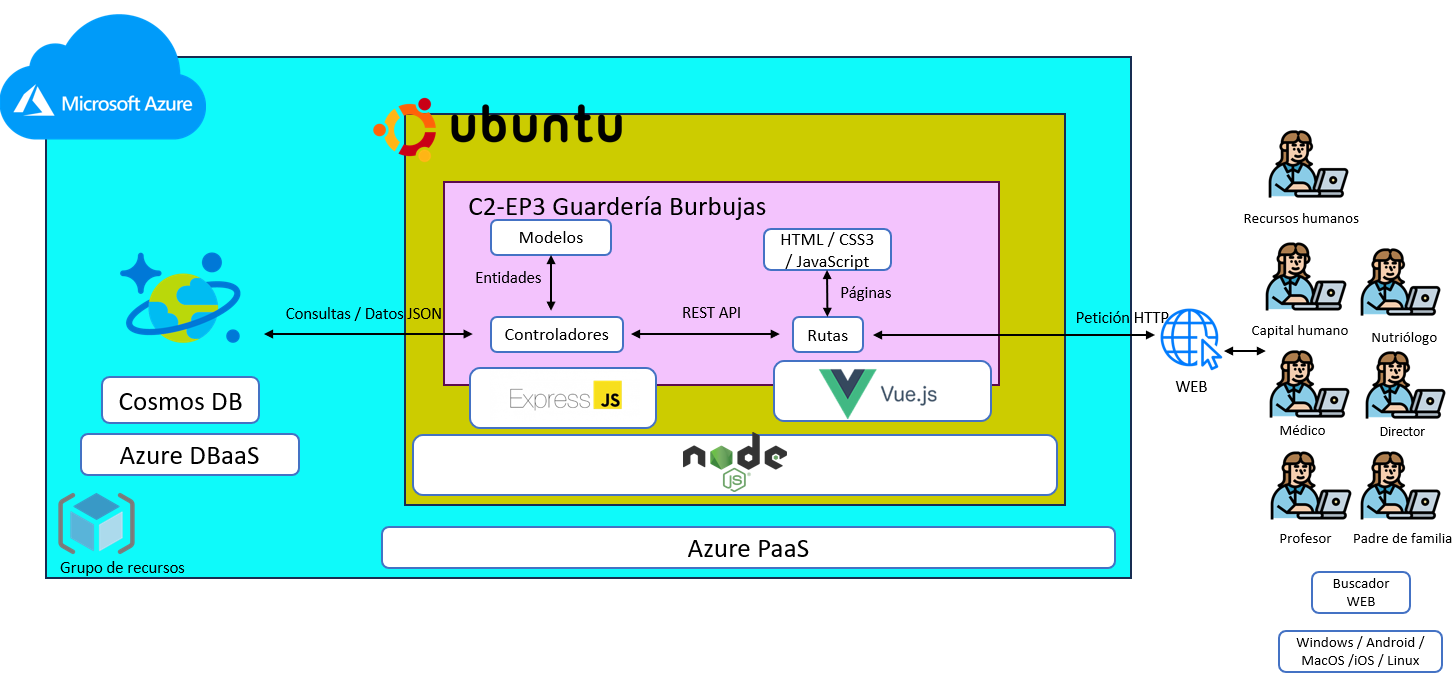
\includegraphics[width=0.9\textwidth]{images/arqui/plataforma.png}
\caption{Plataforma del sistema.}
\label{fig:plataforma}
\end{figure}

%---------------------------------------------------------
\section{Arquitectura.}	

Se puede considerar una arquitectura de tres capas que esta basado en la arquitectura del modelo vista controlador (MVC), que consiste en dividir la aplicación en capas lógicas distintas, cada una con su propósito y responsabilidades específicas. Estas capas son:

\begin{enumerate}
\item Capa de presentación o interfaz de usuario: Esta capa es responsable de la interacción con los usuarios finales y la presentación de la información de manera visualmente atractiva y fácil de usar. En este caso, Vue.js se encarga de construir la interfaz de usuario y proporcionar una experiencia interactiva al usuario. Esta capa también puede incluir la gestión de eventos del lado del cliente y la comunicación con el backend a través de API.

\item Capa de lógica de negocio: Esta capa contiene la lógica y reglas de negocio de la aplicación. Aquí es donde se procesan las solicitudes de los usuarios, se realizan operaciones en la base de datos y se aplican las reglas y validaciones necesarias. En la arquitectura MEVN stack, Express.js se encarga de construir el backend y manejar las solicitudes HTTP, las rutas y la lógica de negocio. En esta capa también se puede implementar la seguridad, la validación de datos y otras funcionalidades relacionadas con la lógica de negocio.

\item Capa de persistencia de datos: Esta capa se encarga del almacenamiento y acceso a los datos. Aquí es donde se interactúa con la base de datos para realizar operaciones de lectura y escritura. En el caso de este sistema, se utiliza Cosmos DB como la base de datos principal. Cosmos DB ofrece una integración nativa con Node.js y permite almacenar y consultar datos de manera eficiente y escalable. En esta capa también se pueden implementar estrategias de caché, gestión de transacciones y otros mecanismos relacionados con la persistencia de datos.

\end{enumerate}

La arquitectura de tres capas proporciona varios beneficios, como la separación de responsabilidades, la modularidad, la reutilización de código y la facilidad de mantenimiento. Cada capa puede desarrollarse y escalarse de forma independiente, lo que permite un desarrollo ágil y una mayor flexibilidad a medida que el sistema evoluciona.

En la Figura \ref{fig:arquitectura-tres-capas} se muestra una representación visual de la arquitectura de tres capas dentro del sistema.

\begin{figure}[htbp]
\centering
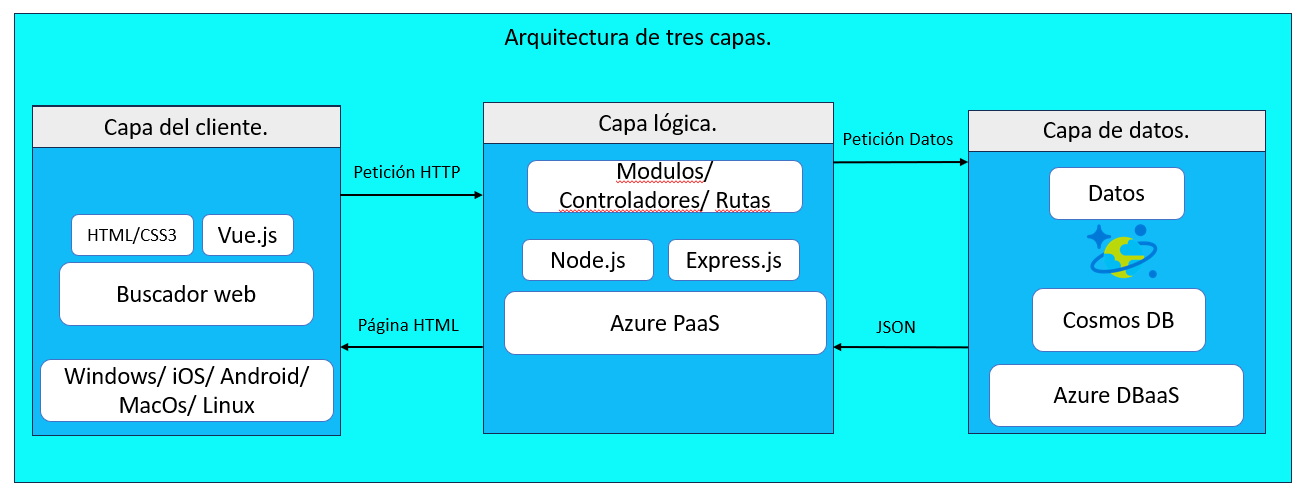
\includegraphics[width=0.9\textwidth]{images/arqui/3capas.png}
\caption{Arquitectura de tres capas en el sistema.}
\label{fig:arquitectura-tres-capas}
\end{figure}

La utilización de la arquitectura MEVN stack junto con la arquitectura de tres capas permite construir un sistema web robusto, escalable y modular. La combinación de estas tecnologías y enfoques arquitectónicos proporciona una base sólida para desarrollar y desplegar aplicaciones web modernas y eficientes en la nube de Azure.